\documentclass[SKL-MASTER.tex]{subfiles}
\begin{document}
	\Large
\section*{Doing Basic Classifications with Decision Trees}
\begin{itemize}
\item In this section we will perform basic classifications using Decision Trees. 
\item These are very nice
models because they are easily understandable, and once trained in, scoring is very simple.
\item Often, SQL statements can be used, which means that the outcome can be used by a lot
of people.
\end{itemize}

\subsection*{Getting Ready}
Decision Trees are the base class
from which a large number of other classification methods are derived. It's a pretty simple
idea that works well in a variety of situations.

\subsection*{Getting Data}
First, let's get some classification data that we can practice on:
\begin{framed}
\begin{verbatim}
>>> from sklearn import datasets
>>> X, y = datasets.make_classification(n_samples=1000, 
   n_features=3, n_redundant=0)
\end{verbatim}
\end{framed}
\subsection{Implementation} %% How to do it…
Working with Decision Trees is easy. We first need to import the object, and then fit the model:
\begin{framed}
\begin{verbatim}
>>> from sklearn.tree import DecisionTreeClassifier
>>> dt = DecisionTreeClassifier()
>>> dt.fit(X, y)

  DecisionTreeClassifier(compute_importances=None, criterion="gini",
  max_depth=None, max_features=None,
  max_leaf_nodes=None, min_density=None,
  min_samples_leaf=1, min_samples_split=2,
  random_state=None, splitter='best')
  
>>> preds = dt.predict(X)
>>> (y == preds).mean()
   1.0
\end{verbatim}
\end{framed}


\begin{figure}
\centering
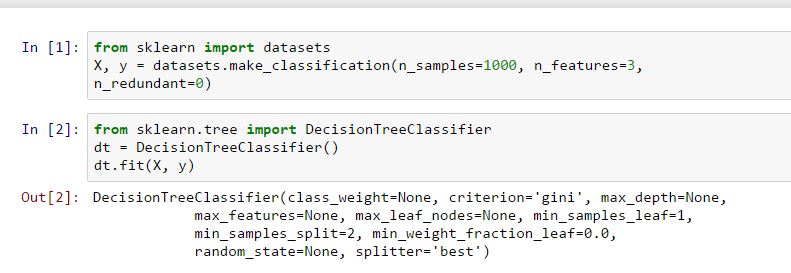
\includegraphics[width=0.7\linewidth]{images/SKL41-DT1}

\end{figure}
%
%As you can see, we guessed it right. Clearly, this was just a dry run, now let's investigate some
%of our options.
%===================================================%
% % Chapter 4
% % 121
First, if you look at the \texttt{dt} object, it has several keyword arguments that determine how the
object will behave. How we choose the object is important, so we'll look at the object's effects
in detail.
\subsection*{Maximum Depth}
\begin{itemize}
\item The first detail we'll look at is \texttt{max\_depth}. This is an important parameter. It determines how
many branches are allowed. 
\item This is important because a Decision Tree can have a hard time
generalizing out-of-sampled data with some sort of regularization. 
\item Later, we'll see how we
can use several shallow Decision Trees to make a better learner. 
\item Let's create a more complex
dataset and see what happens when we allow different \texttt{max\_depth}. We'll use this dataset for
the rest of the exercise:
\end{itemize}
{
	\Large
\begin{framed}
\begin{verbatim}
>>> n_features=200
>>> X, y = datasets.make_classification(750,
n_features,n_informative=5)
>>> import numpy as np
>>>
>>> training = np.random.choice([True, False], 
p=[.75, .25],size=len(y))
>>
>>> accuracies = []
>>>
>>> for x in np.arange(1, n_features+1):
>>> dt = DecisionTreeClassifier(max_depth=x)
>>> dt.fit(X[training], y[training])
>>> preds = dt.predict(X[~training])
>>> accuracies.append((preds == y[~training]).mean())
\end{verbatim}
\end{framed}
}
\begin{framed}
	\begin{verbatim}
>>> import matplotlib.pyplot as plt
>>> f, ax = plt.subplots(figsize=(7, 5))
>>> ax.plot(range(1, n_features+1), accuracies, color='k')
>>> ax.set_title("Decision Tree Accuracy")
>>> ax.set_ylabel("% Correct")
>>> ax.set_xlabel("Max Depth")
\end{verbatim}
\end{framed}
%===================================================%
% % Classifying Data with scikit-learn
% % 122

\begin{figure}[h!]
\centering
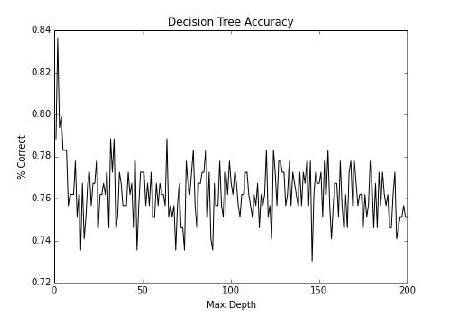
\includegraphics[width=0.7\linewidth]{images/SKL33-DT2}
\end{figure}


We can see that we actually get pretty accurate at a low max depth. Let's take a closer look at
the accuracy at low levels, say the first 15:
\begin{framed}
\begin{verbatim}
>>> N = 15
>>> import matplotlib.pyplot as plt
>>> f, ax = plt.subplots(figsize=(7, 5))
>>> ax.plot(range(1, n_features+1)[:N], accuracies[:N], color='k')
>>> ax.set_title("Decision Tree Accuracy")
>>> ax.set_ylabel("% Correct")
>>> ax.set_xlabel("Max Depth")
\end{verbatim}
\end{framed}
%===================================================%
% % Chapter 4
% % 123
The following is the output:

\begin{figure}
\centering
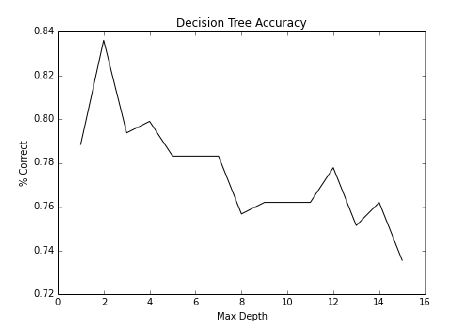
\includegraphics[width=0.7\linewidth]{images/SKL33-DT3}
\caption{}
\label{fig:SKL33-DT3}
\end{figure}

There's the spike we saw earlier; it is interesting to see the quick drop though. It's more
likely that Max Depth of 1 through 3 is fairly equivalent. Decision Trees are quite good at
separating rules, but they need to be reigned in.
We'll look at the \texttt{compute\_importances} parameter here. It actually has a bit of a broader
meaning for random forests, but we'll get acquainted with it.

% It's also worth noting that if you're using Version 0.16 or earlier, you will get this for free:
\begin{framed}
\begin{verbatim}
>>> dt_ci = DecisionTreeClassifier(compute_importances=True)
>>> dt.fit(X, y)
\end{verbatim}
\end{framed}
%===================================================%
Plot the importances

\begin{framed}
\begin{verbatim}
>>> ne0 = dt.feature_importances_ != 0
>>> y_comp = dt.feature_importances_[ne0]
>>> x_comp = np.arange(len(dt.feature_importances_))[ne0]
>>>
>>> import matplotlib.pyplot as plt
>>> f, ax = plt.subplots(figsize=(7, 5))
>>> ax.bar(x_comp, y_comp)
\end{verbatim}
\end{framed}
%===================================================%
% % Classifying Data with scikit-learn
% % 124
The following is the output:

\begin{figure}
\centering
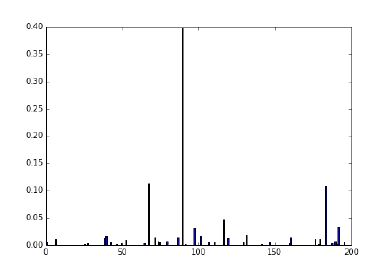
\includegraphics[width=0.7\linewidth]{images/SKL33-DT4}
\caption{}
\label{fig:SKL33-DT4}
\end{figure}

\begin{itemize}
\item Please note that you may get an error letting you know you'll
no longer need to explicitly set compute importances.
\item As we can see, one of the features is by far the most important; several other features will
follow up.
\end{itemize}
\newpage
%===================================================%
\subsection*{Theoretical Aspects}
\begin{itemize}

\item In the simplest sense, we construct Decision Trees all the time. 
\item When thinking through
situations and assigning probabilities to outcomes, we construct Decision Trees. 
\item Our rules
are much more complex and involve a lot of context, but with Decision Trees, all we care
about is the difference between outcomes, given that some information is already known
about a feature.
\end{itemize}

\subsection*{Information Gain and Gini Impurity}
\begin{itemize}
\item Now, let's discuss the differences between entropy and Gini impurity.
\item Entropy is more than just the entropy value at any given variable; it states what the change in
entropy is if we know an element's value. 
\item This is called Information Gain (IG); mathematically
it looks like the following:
\[\mbox{IG(Data, Known Features) }= H (Data)- H (Data|Known Features)\]
\item For Gini impurity, we care about how likely one of the data points will be mislabeled given the
new information.

\item Both entropy and Gini impurity have pros and cons; this said, if you see major differences
in the working of entropy and Gini impurity, it will probably be a good idea to re-examine
your assumptions.
\end{itemize}

%===================================================%
%% Chapter 4
%% 125
\newpage
\section*{Tuning a Decision Tree model}
If we use just the basic implementation of a Decision Tree, it will probably not fit very well.
Therefore, we need to tweak the parameters in order to get a good fit. This is very easy and
won't require much effort.
\subsection*{Getting Ready}
\begin{itemize}
\item In this exercise, we will take an in-depth look at what it takes to tune a Decision Tree classifier.
\item There are several options, and in the previous recipe, we only looked at one of these options.
\item We'll fit a basic model and actually look at what the Decision Tree looks like. 
\item Then,
we'll re-examine after each decision and point out how various changes have influenced
the structure.
\item If you want to follow along in this exercise, you'll need to install \textbf{pydot}.
\end{itemize}

\subsection*{Implementation}
Decision Trees have a lot more "knobs" when compared to most other algorithms, because of
which it's easier to see what happens when we turn the knobs:
\begin{framed}
\begin{verbatim}
>>> from sklearn import datasets
>>> X, y = datasets.make_classification(1000, 20, n_informative=3)
>>> from sklearn.tree import DecisionTreeClassifier
>>> dt = DecisionTreeClassifier()
>>> dt.fit(X, y)
\end{verbatim}
\end{framed}
%===================================================%
Ok, so now that we have a basic classifier fit, we can view it quite simply:
\begin{framed}
\begin{verbatim}
>>> from StringIO import StringIO
>>> from sklearn import tree
>>> import pydot
>>> str_buffer = StringIO()
>>> tree.export_graphviz(dt, out_file=str_buffer)
>>> graph = pydot.graph_from_dot_data(str_buffer.getvalue())
>>> graph.write("myfile.jpg")
\end{verbatim}
\end{framed}
%===================================================%
% % Classifying Data with scikit-learn
% % 126
The graph is almost certainly illegible, but hopefully this illustrates the complex trees that can
be generated as a result of using an unoptimized decision tree:
%===================================================%
% % Chapter 4
% % 127
%% Wow! 
This is a very complex tree. It will most likely overfit the data. First, let's reduce the max
depth value:
\begin{framed}
\begin{verbatim}
>>> dt = DecisionTreeClassifier(max_depth=5)
>>> dt.fit(X, y);
\end{verbatim}
\end{framed}
As an aside, if you're wondering why the semicolon, the repr by default, is seen, it is actually
the model for a Decision Tree. For example, the fit function actually returns the Decision
Tree object that allows chaining:
\begin{framed}
\begin{verbatim}
>>> dt = DecisionTreeClassifier(max_depth=5).fit(X, y)
\end{verbatim}
\end{framed}
Now, let's get back to the regularly scheduled program.
As we will plot this a few times, let's create a function:
\begin{framed}
\begin{verbatim}
>>> def plot_dt(model, filename):
str_buffer = StringIO()
>>> tree.export_graphviz(model, out_file=str_buffer)
>>> graph = pydot.graph_from_dot_data(str_buffr.getvalue())
>>> graph.write_jpg(filename)
>>> plot_dt(dt, "myfile.png")
\end{verbatim}
\end{framed}
%===================================================%
% % Classifying Data with scikit-learn
% % 128
The following is the graph that will be generated:
%===================================================%
% % Chapter 4
% % 129
This is a much simpler tree. Let's look at what happens when we use entropy as the
splitting criteria:
\begin{framed}
\begin{verbatim}
>>> dt = DecisionTreeClassifier(criterion='entropy',
max_depth=5).fit(X, y)
>>> plot(dt, "entropy.png")
\end{verbatim}
\end{framed}
The following is the graph that can be generated:
%===================================================%
% % Classifying Data with scikit-learn
% % 130
It's good to see that the first two splits are the same features, and the first few after this are
interspersed with similar amounts. This is a good sanity check.
Also, note how entropy for the first split is 0.999, but for the first split when using the Gini
impurity is 0.5. This has to do with how different the two measures of the split of a Decision
Tree are. 

% % See the following How it works... section for more information. 
However, if we want
to create a Decision Tree with entropy, we must use the following command:
\begin{framed}
\begin{verbatim}
>>> dt = DecisionTreeClassifier(min_samples_leaf=10,
criterion='entropy',
max_depth=5).fit(X, y)
\end{verbatim}
\end{framed}
%------------------------------------------%
\subsubsection*{Overfitting}
\begin{itemize}
\item Decision Trees, in general, suffer from overfitting. Quite often, left to it's own devices, a
Decision Tree model will overfit, and therefore, we need to think about how best to avoid
overfitting; this is done to avoid complexity. 
\item A simple model will more often work better in
practice than not.
\item We're about to see this very idea in practice. random forests will build on this idea of
simple models.
\end{itemize}
\end{document}
